% VDE Template for EUSAR Papers
% Provided by Barbara Lang und Siegmar Lampe
% University of Bremen, January 2002
% English version by Jens Fischer
% German Aerospace Center (DLR), December 2005
% Additional modifications by Matthias Wei{\ss}
% FGAN, January 2009

%-----------------------------------------------------------------------------
% Type of publication
\documentclass[a4paper,10pt]{article}
%-----------------------------------------------------------------------------
% Other packets: Most packets may be downloaded from www.dante.de and
% "tcilatex.tex" can be found at (December 2005):
% http://www.mackichan.com/techtalk/v30/UsingFloat.htm
% Not all packets are necessarily needed:
\usepackage[T1]{fontenc}
\usepackage[latin1]{inputenc}
%\usepackage{ngerman} % in german language if required
\usepackage[nooneline,bf]{caption} % Figure descriptions from left margin
\usepackage{times}
\usepackage{multicol}
\usepackage{amsmath}
\usepackage{amssymb}
\usepackage[dvips]{graphicx}
\usepackage{epsfig}
\usepackage[usenames,dvipsnames]{xcolor}
\usepackage{pstricks}
\usepackage{wrapfig}
\usepackage{epstopdf}
\usepackage{tabularx}
\input{tcilatex}
%-----------------------------------------------------------------------------
% Page Setup
\textheight24cm \textwidth17cm \columnsep6mm
\oddsidemargin-5mm                 % depending on print drivers!
\evensidemargin-5mm                % required margin size: 2cm
\headheight0cm \headsep0cm \topmargin0cm \parindent0cm
\pagestyle{empty}                  % delete footer and header
%----------------------------------------------------------------------------
%hyperref
\usepackage[breaklinks]{hyperref}
\hypersetup{
	bookmarks=true,         % show bookmarks bar?
	pdftoolbar=true,        % show Acrobat’s toolbar?
	pdfmenubar=true,        % show Acrobat’s menu?
	pdffitwindow=false,  
	pdftitle={Android Open ADK on iNEMO platform},    % title
	pdfauthor={Gianazza Andrea},     	 % author
	pdfsubject={Demo application showing the support of Android ADK to STM32 microcontrollers family},
	pdfkeywords={STM} {ADK} {Android} {Embedded Systems}
}
%----------------------------------------------------------------------------
% Environment definitions
\newenvironment*{mytitle}{\begin{LARGE}\bf}{\end{LARGE}\\}%
\newenvironment*{mysubtitle}{\bf}{\\[1.5ex]}%
\newenvironment*{myabstract}{\begin{Large}\bf}{\end{Large}\\[2.5ex]}%
%-----------------------------------------------------------------------------
% Using Pictures and tables:
% - Instead "table" write "tablehere" without parameters
% - Instead "figure" write "figurehere " without parameters
% - Please insert a blank line before and after \begin{figuerhere} ... \end{figurehere}
%
% CAUTION:   The first reference to a figure/table in the text should be formatted fat.
%
\makeatletter
\newenvironment{tablehere}{\def\@captype{table}}{}
\newenvironment{figurehere}{\def\@captype{figure}\vspace{2ex}}{\vspace{2ex}}
\def\hlinewd#1{%
\noalign{\ifnum0=`}\fi\hrule \@height #1 %
\futurelet\reserved@a\@xhline}
\makeatother

\renewcommand{\arraystretch}{1.2}

%%%%%%%%%%%%%%%%%%%%%%%%%%%%%%%%%%%%%%%%%%%%%%%%%%%%%%%%%%%%%%%%%%%%%%%%%%%%%%
\begin{document}

% Please use capital letters in the beginning of important words as for example
\begin{mytitle}Android Open ADK on iNEMO platform\end{mytitle}
\begin{mysubtitle}Demo application showing the support of Android Open ADK to STM32 microcontrollers' family\end{mysubtitle}
%
% Please do not insert a line here
%
\\
Gianazza Andrea\\
Matr. 755119, (g.gianazza87@gmail.com)\\
\hspace{10ex}
Scolari Alberto\\
Matr. 123456, (al.scolari@alice.it)\\
\hspace{10ex}
Turri Matteo\\
Matr. 123456, (matteoturri89@gmail.com)\\
\begin{flushright}
\emph{Report for the master course of Embedded Systems}\\
\emph{Reviser: PhD. Patrick Bellasi (bellasi@elet.polimi.it)}
\end{flushright}

Received: \today \\
\hspace{10ex}

\begin{myabstract} Abstract \end{myabstract}
In 2011 Google presented the Android Open Accessory Development Kit (ADK), a software framework that allows external USB hardware to easily communicate with Android-powered devices. Several distributors started to produce Android Open Accessory compatible development boards, in order to promote the diffusion of USB accessories for Android. The aim of this work is to show the support of Android Open ADK to STM32 microcontrollers family, porting the Windows iNEMO demo application to Android.

\vspace{4ex}	% Please do not remove or reduce this space here.
\begin{multicols}{2}

%%%%%%%%%%%%%%%%%%%%%%%%%%%%%%%%%%%%%%%%%%%%%%%%%%%%%%%%%%%%%%%%%%%%%%%%%%%%%

\section{Introduction}
\label{intro}

During the Google I/O 2011 conference, Google announced the Android Open Accessory APIs for Android. These APIs allow USB accessories to connect to Android devices running Android 3.1 or Android 2.3.4 without special licensing or fees. The new ``Accessory mode'' does not require the Android device to support USB Host mode. In accessory mode the Android phone or tablet acts as the USB Device and the accessory acts as the USB Host. Hence, Android Open ADK opens up the possibility to easily realize a set of new accessories fully compatible with Android-powered devices that do not support USB Host functionality. For this reason, several distributors started to produce Android Open Accessory compatible development boards, in order to promote the diffusion of this type of accessories. The aim of this work is to add the support of the Android Open ADK to STM32 microcontrollers' family and to develop a demo application in order to show how this protocol can be used. The iNEMOv2 board has been chosen as the target platform for this test case: the goal is to realize the porting of the Windows application iNEMO Suite to Android.

The document is organized in six sections. After this short introduction, an overview on the hardware setup is provided in Section \ref{hw_sec}. Section \ref{adk_sec} describes the main features of the Android Accessory protocol. The Communication Protocol adopted is described in Section \ref{cp_sec}. Section \ref{sw_sec} is focused on the descrition of the key points of the firmware and of the Android application developed. Finally Section \ref{conclusions} discusses the obtained results and the next steps that will be achieved in future.

Source code and documentation for this work are freely accessible from the GIT repository located at \url{http://code.google.com/p/stm32-adk/}. 

\section{Hardware Overview}
\label{hw_sec}

This section describes the hardware setup needed for enabling Android Open ADK on STM32-based kits. In particular, STEVAL-MKI062V2 (iNEMO) \cite{STM_inemo} board has been used in this demo application, but the work presented can be easily adapted to whatever STM32 based board. The STEVAL-MKI062V2 is the second generation of the iNEMO module family. It combines accelerometers, gyroscopes and magnetometers with pressure and temperature sensors to provide 3-axis sensing of linear, angular and magnetic motion, complemented with temperature and barometer/altitude readings, offering in this way a 10 degrees of freedom (DOF) platform. More specifically, the board integrates five STMicroelectronics sensors: a 2-axis roll-and-pitch gyroscope, a 1-axis yaw gyroscope, a 6-axis geomagnetic module, a pressure sensor, and a temperature sensor (see {\bf Figure \ref{fig:inemov2}}).

\begin{center}
	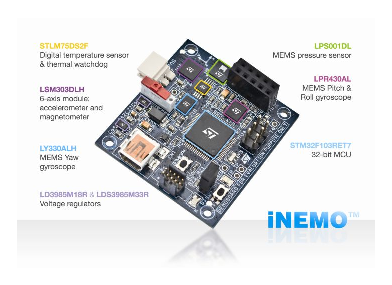
\includegraphics[width=0.95\linewidth]{pics/inemov2.eps}
	\captionof{figure}{iNEMO V2 platform.}
	\label{fig:inemov2}
\end{center}

As we said, the communication between the board and the Android device is realized using the Android Open ADK: according to this protocol the iNEMO acts as the USB host (powers the bus and enumerates devices) and the Android-powered device acts as the USB device (see section \ref{adk_sec} for more details). Since the iNEMO does not natively integrate a USB port, it is necessary to use a USB Host Shield in order to provide USB Host functionality to the board. In this work it has been used the USB Host Shield furnished by Sparkfun\footnote{Sparkfun USB Host Shield: \url{http://www.sparkfun.com/products/9947}}, but whatever equivalent board offering Maxim MAX3421E\cite{max3421e} USB host controller can be adopted. The iNEMO board communicates with the Host Shield through a Serial Peripheral Interface (SPI) bus: as a matter of fact, the Extended Connector (J8) of the iNEMO provides an SPI interface and 4 GPIOs (see {\bf Figure \ref{fig:j8}}) that can be used to control the Shield.

\begin{center}
	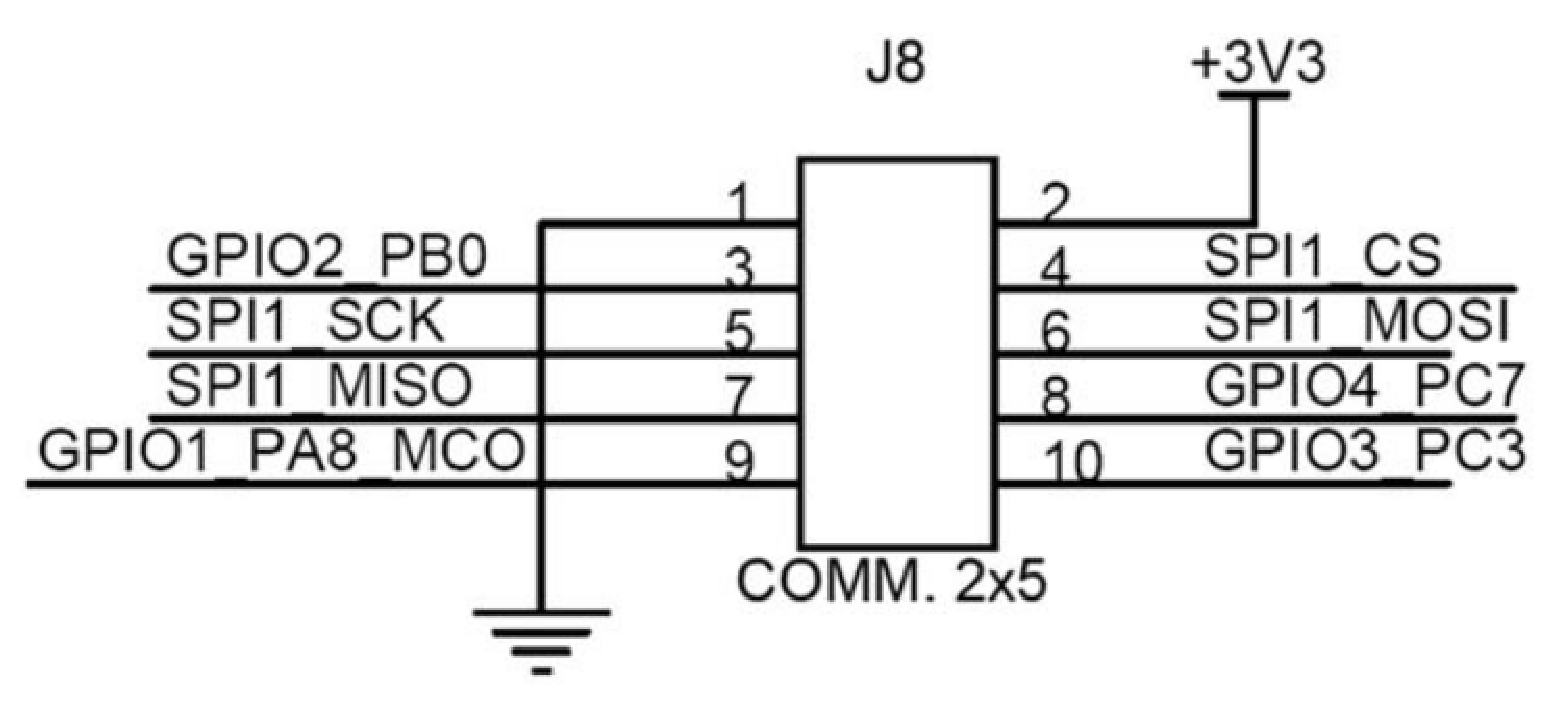
\includegraphics[width=0.95\linewidth]{pics/j8.eps}
	\captionof{figure}{Extended Connector (J8) schematic.}
	\label{fig:j8}
\end{center}

The connections between the iNEMO board and the USB Host Shield are shown in {\bf Figure \ref{fig:spi}}. This picture shows also that the Shield must be powered by means of an external power supply (9V) on VIn pin.

\begin{center}
	\includegraphics[width=0.95\linewidth]{pics/SPI_wirings.eps}
	\captionof{figure}{Connections between the iNEMO board and the USB Host Shield.}
	\label{fig:spi}
\end{center}

For debugging purposes, a TTL-232R-PCB by FTDI\cite{ttl232r} has been connected to the 6-pin COM J4 connector of the iNEMO board.

{\bf Figure \ref{fig:connections}} shows an overview of the components used in this work and the connections between them.

\begin{center}
	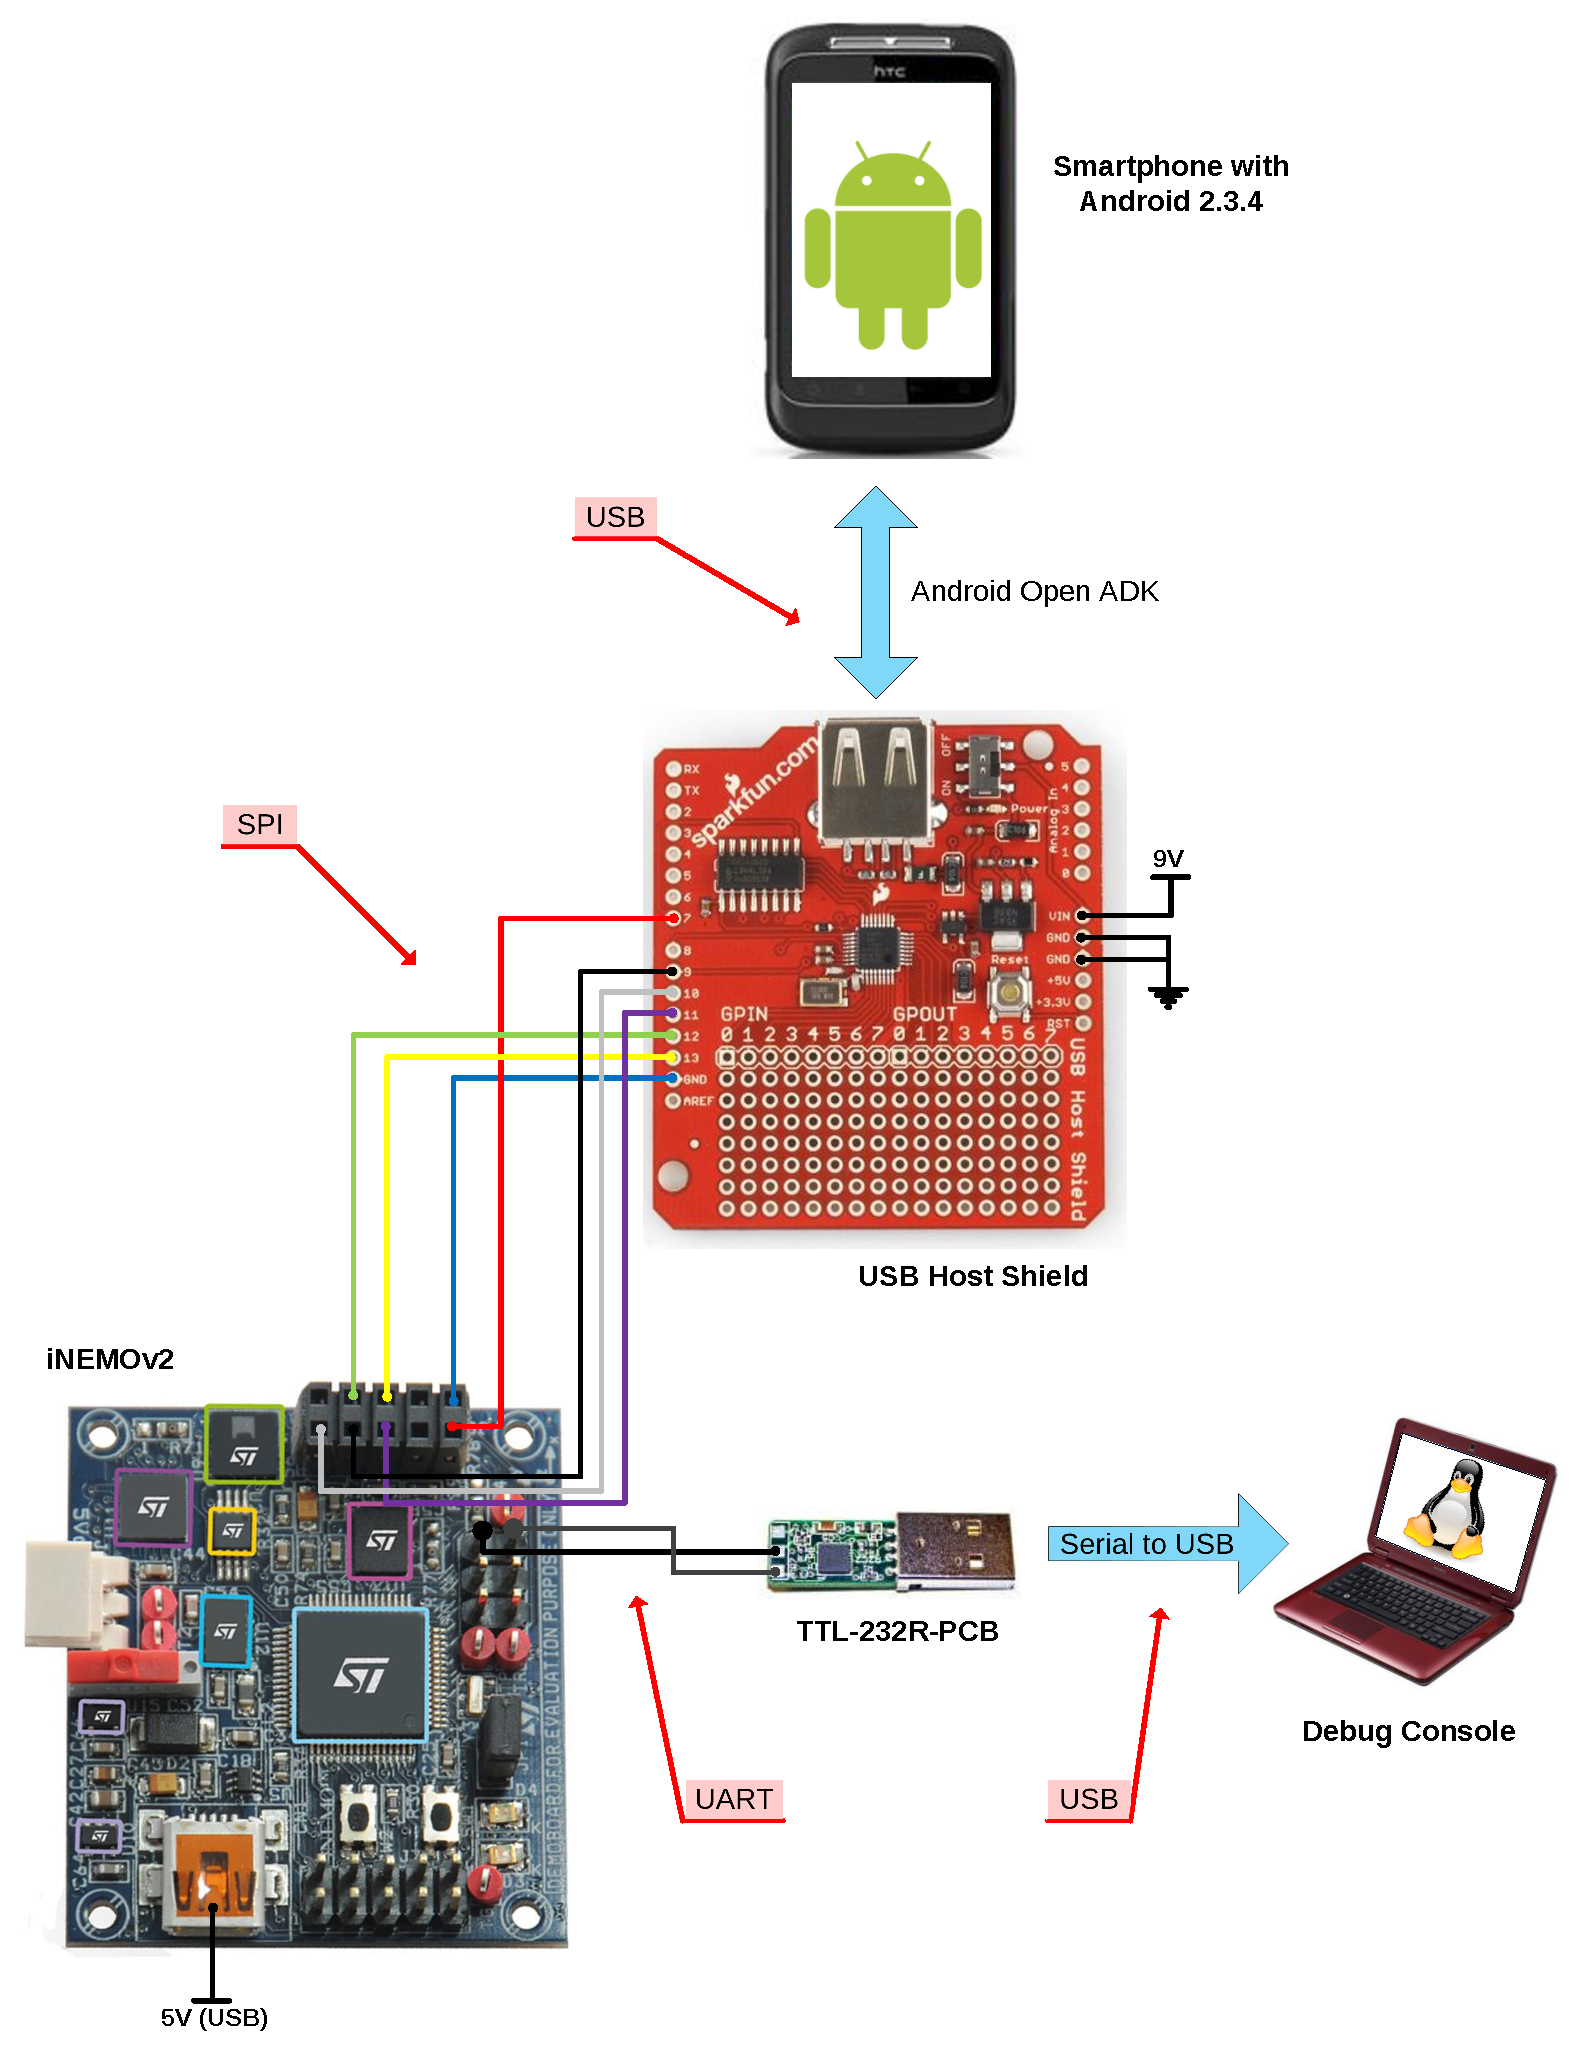
\includegraphics[width=0.95\linewidth]{pics/connections.eps}
	\captionof{figure}{Overview of the hardware used.}
	\label{fig:connections}
\end{center}


\section{Android Open ADK}
\label{adk_sec}

The iNEMO board and the Android-powered device communicate on a USB bus. USB is an asymmetric protocol in that one participant acts as a USB Host and all other participants are USB Devices. The USB Host has two important tasks. The first is to be the bus master and control which device sends data at what times. The second key task is to provide power, since USB is a powered bus (see {\bf Figure \ref{fig:usb_normal}}). The problem with supporting accessories on Android in the traditional way is that relatively few devices support Host mode. Android Open ADK offers an answer to this problem, inverting the normal USB relationship.

\begin{center}
	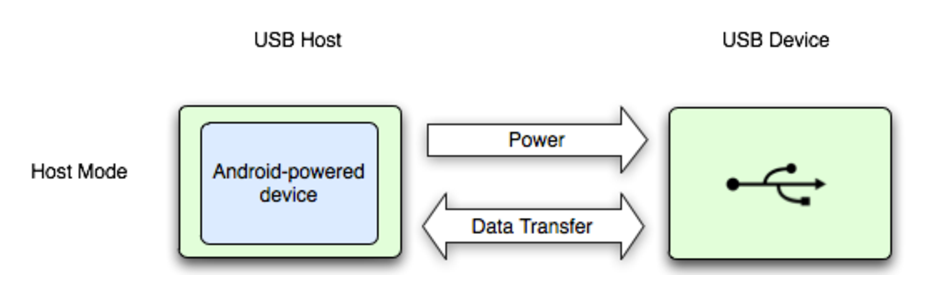
\includegraphics[width=1\linewidth]{pics/usb_normal.eps}
	\captionof{figure}{Normal USB relationship.}
	\label{fig:usb_normal}
\end{center}

During the Google I/O 2011 conference, Google announced the Android Open Accessory APIs for Android. These APIs allow USB accessories to connect to Android devices running Android 3.1 or Android 2.3.4 without special licensing or fees. The new ``accessory mode'' does not require the Android device to support USB Host mode. In accessory mode the Android phone or tablet acts as the USB Device and the accessory acts as the USB Host. This means that the accessory is the bus master and provides power (see {\bf Figure \ref{fig:usb_accessory}}).

\begin{center}
	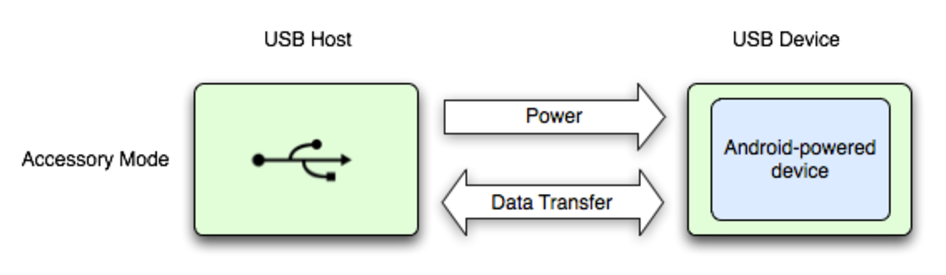
\includegraphics[width=1\linewidth]{pics/usb_accessory.eps}
	\captionof{figure}{Inverted USB relationship: the accessory acts as the USB host.}
	\label{fig:usb_accessory}
\end{center}

Building an Open Accessory is quite simple, as the only HW requirements are to include a USB host and provide power to the Android device. The accessory needs to implement a simple handshake to establish a bi-directional connection with an application running on the Android device.

The handshake starts when the accessory detects that a device has been connected to it. The Android device will identify itself with the VID/PID that are defined by the manufacturer and the model of the device. The accessory then sends a control transaction to the Android device asking if it supports accessory mode.

Once the accessory confirms the Android device supports accessory mode, it sends a series of strings to the Android device using control transactions. These strings allow the Android device to identify compatible applications as well as provide a URL that Android will use if a suitable app is not found. Next the accessory sends a control transaction to the Android device telling it to enter accessory mode.

The Android device then drops off the bus and reappears with a new VID/PID combination. The new VID/PID corresponds to a device in accessory mode, which is Google's VID 0x18D1, and PID 0x2D01 or 0x2D00. Once an appropriate application is started on the Android side, the accessory can now communicate with it using the first Bulk IN and Bulk OUT endpoints.

The protocol is quite easy to implement on the accessory: a complete tutorial on the implementation of Open ADK can be found in the USB section of the official Android Developer's Guide\footnote{Android Developer's Guide: \url{http://developer.android.com/guide/index.html}}.


\section{Communication Protocol}
\label{cp_sec}

As said in section \ref{adk_sec}, Android Open ADK allows the accessory to exchange generic data with the Android device. A communication protocol is needed to structure this data, in order to allow iNEMO board to correctly communicate with the Android device. At the beginning of this work we had two options for the choice of the protocol:

\begin{itemize}
	\item define a brand new protocol, maybe taking a cue from OpenDMTP\footnote{The OpenDMTP Project: \url{http://www.opendmtp.org}};
	\item adapting the original protocol defined by STM for the communication with the Windows application INEMO Suite.
\end{itemize}

We think that the second option is the best one for the following reasons:

\begin{itemize}
	\item it allows to maintain a continuity whit what has already been developed by STMicroelectronics;
	\item the original protocol is designed to best exploit the features of the board and to fit into the libraries written for it;
	\item it is not useful to write a new protocol that makes the same things that the original one does, but simply with a different format for the exchanged messages.
\end{itemize}

Therefore, an overview of the original protocol is now presented. The messages exchanged by the board have a standard frame that can be described as a sequence of fields in a specific order. The frame format is composed of a header and an optional payload. The header is composed of three mandatory (M) fields, each of which is 1 byte in length, while the payload is an optional field whose maximum length is 61 bytes (this limit can be exceeded by setting the LF/MF field, as explained below). {\bf Figure \ref{fig:frame_format}} shows the general frame format. 

\begin{center}
	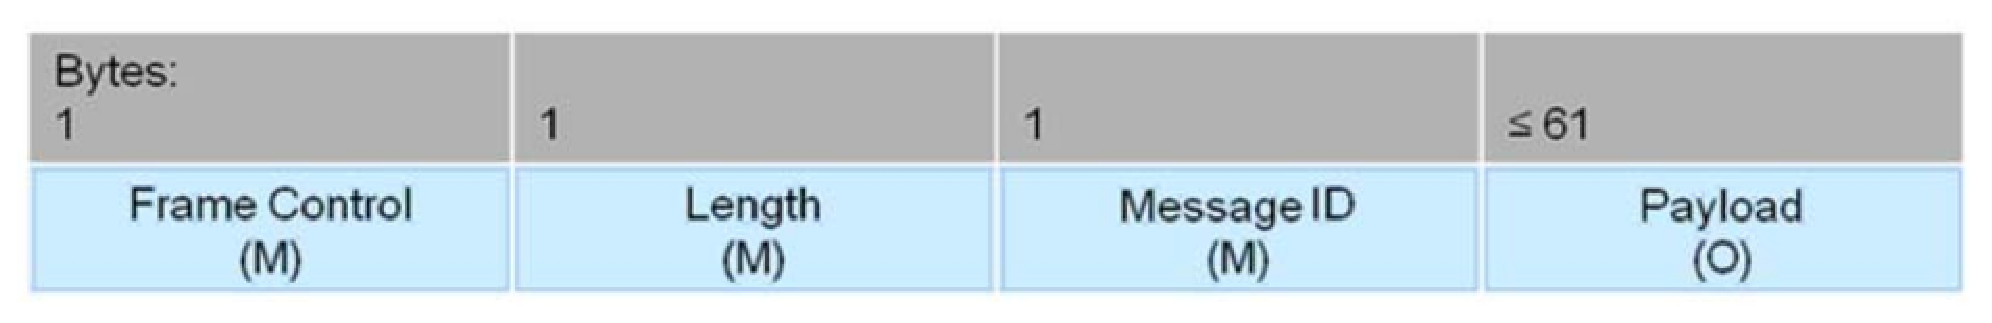
\includegraphics[width=1\linewidth]{pics/frame_format.eps}
	\captionof{figure}{General frame format.}
	\label{fig:frame_format}
\end{center}

The frame control field is 1 byte in length and contains information defining the frame type and other control flags (see {\bf Figure \ref{fig:control_field}}).

\begin{center}
	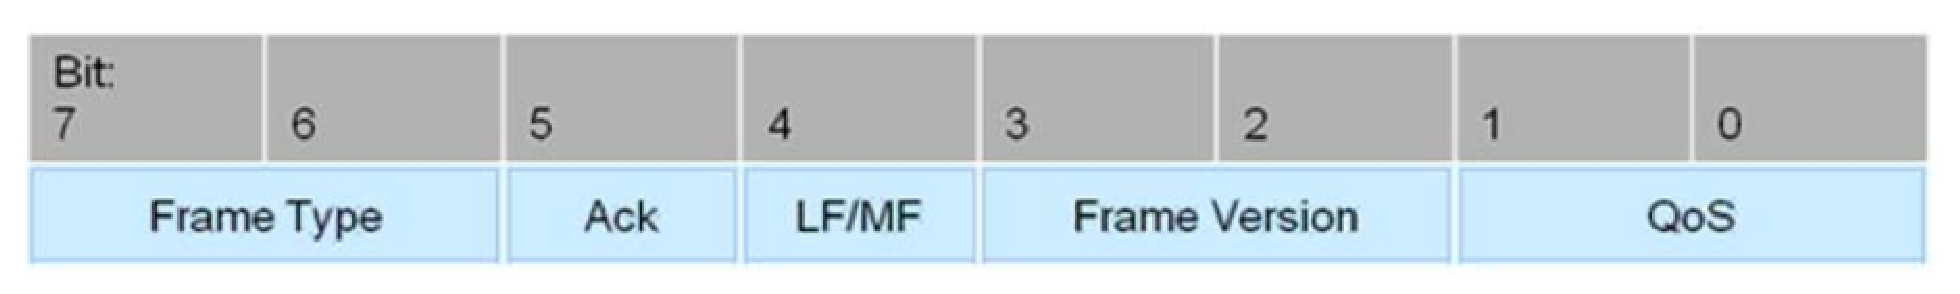
\includegraphics[width=1\linewidth]{pics/control_field.eps}
	\captionof{figure}{Frame control field.}
	\label{fig:control_field}
\end{center}

The frame type subfield is 2 bits in length and is set to one of the values listed in {\bf Table \ref{tab:frame_list}}.

\begin{center}
	\begin{tabularx}{0.9\linewidth}{|>{\centering\arraybackslash}X|>{\centering\arraybackslash}X|}
		\hline
		\textbf{Value} & \textbf{Frame Type} \\
		\hlinewd{1.5pt}
		00 & CONTROL \\
		\hline		
		01 & DATA \\
		\hline
		10 & ACK \\
		\hline
		11 & NACK \\
		\hline
	\end{tabularx}
	\captionof{table}{Frame type list}
	\label{tab:frame_list}
\end{center}

The ACK subfield is 1 bit in length and specifies whether an acknowledgement is required from the recipient on receipt of a DATA or CONTROL frame. If this field is set to one, the recipient sends an acknowledgment frame only if, upon reception, the frame passes all required levels of filtering. If this subfield is set to zero, the recipient device does not send an acknowledgment frame. It is possible to embed a payload in an acknowledgment frame (piggybacking) to send useful information to the transmitter and avoid further transactions. When the ACK field is set to one, and if, upon reception, the frame does not pass the required level of filtering, the recipient sends a no-acknowledgment frame (NACK), whose payload is an error code (e.g. unsupported command, value out of range,...). In the ACK and/or NACK frames the ACK field is set to zero and ignored upon reception.

The LF/MF (last fragment / more fragment) subfield is 1 bit in length and it is used for fragmentation and reassembling. This field is set to zero to indicate a single frame or the last frame of a multiple-frame transaction. This field is set to 1 to indicate that other frames follow, all belonging to the same transaction. 

The frame version subfield is 2 bits in length and is set to ``00'' at this time.

The QoS (Quality of Service) subfield is 2 bits in length and is set to one of the values listed in {\bf Table \ref{tab:qos_list}}. This subfield allows the application to exchange and process data and control frames with different priorities.

\begin{center}
	\begin{tabularx}{0.9\linewidth}{|>{\centering\arraybackslash}X|>{\centering\arraybackslash}X|}
		\hline
		\textbf{Value} & \textbf{QoS} \\
		\hlinewd{1.5pt}
		00 & Normal Priority \\
		\hline		
		01 & Medium Priority \\
		\hline
		10 & High Priority \\
		\hline
	\end{tabularx}
	\captionof{table}{Frame type list}
	\label{tab:qos_list}
\end{center}

Returning to the frame format, the length field is 1 byte in length and contains the number of bytes that follow. Admitted values are in the range 1 to 62.

The message ID is 1 byte in length and contains an identifier used to distinguish the messages.


The frames are classified in four types:

\begin{enumerate}
	\item Communication control frames.
	\item Board information frames.
	\item Sensor setting frames.
	\item Acquisition sensor data frames.
\end{enumerate}

A detailed description of the different frames can be found in the documentation about the Communication Protocol provided by STMicroelectronics\cite{STM_protocol}.




\section{Software Overview}
\label{sw_sec}

This section presents an overview of the firmware developed for the iNEMO board and the application developed for the Android device.

\subsection{Firmware}
\label{fw_sec}

The firmware for the iNEMO board is based on the real-time operating system FreeRTOS, version 7\footnote{The FreeRTOS Project: \url{http://www.freertos.org}}. Most of the code is taken from the original code furnished by STMicroelectronics: in particular, the libraries to manage sensors, ports and internal communication have been totally reused without any change. The main contributes to the firmware of this work are the support of Android Open ADK and the implementation of a set of tasks to allow communication with the Android device.

As said in section \ref{hw_sec}, USB Host functionality is provided by an USB Host Shield that integrates the Maxim MAX3421E USB host controller. Hence, to support the communication on the USB through the MAX3421E, USB control library and MAX3421E driver, developed by Circuits@Home\footnote{Circuits@Home: \url{http://www.circuitsathome.com}} for the Arduino Platform, have been adapted to STM32 microcontrollers family. At the higher level of the software stack there is the Android Accessory library: it has been implemented according to the indications furnished by the Android Developer's Guide. {\bf Figure \ref{fig:sw_stack}} shows the software stack for the support of Android Open ADK. 

\begin{center}
	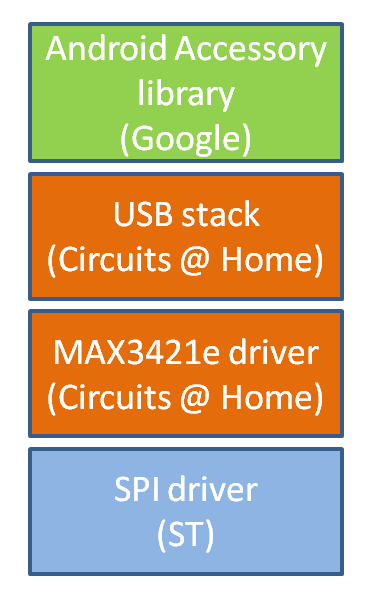
\includegraphics[width=0.5\linewidth]{pics/sw_stack.eps}
	\captionof{figure}{Software stack for the support of Android Open ADK.}
	\label{fig:sw_stack}
\end{center}

The communication with the Android device is guaranteed by 3 tasks:

\begin{itemize}
 	\item Accessory Task: it manages the communication according to the Accessory protocol and can awake the Command Task in order the process the messages received from the Android device.
	\item Command Task: it parses the messages received from the Android device and builds the response messages. It can awake the Data Task.
	\item Data Task: it sends messages containing data received from the sensors integrated on the board.
\end{itemize}  

The Accessory task is always active: it examines the USB bus to check if an Android device is attached. In case a device is found, the Accessory Task establishes a connection with it (see section \ref{adk_sec}). Once the device is in Accessory mode, the Accessory Task waits for messages from it. When a message is received, it is sent to the queue on which the Command Task is waiting for. Then, the Command Task can retrieve the message sent from the device and parse it. According to the contents of the message, the Command Task sends an appropriate response message and eventually enables or disables the Data Task. When enabled, the Data Task sends the data retrieved from the sensors of the board to the Android device.

Keil uVision 4 has been used as development environment and debugger for the realization of the firmware. The main issue encountered in using this IDE was the limitation on the code size (32KB) present in the free version (MDK-Lite): this forced us to eliminate, for the moment, the support of gyroscopes, magnetometer and pressure sensor, even if the libraries for them are ready to be used. For this reason, one of the future goal for this work is to implement a completely open compile chain (probably based on gcc), in order to get rid of the limitations imposed by Keil uVision IDE.

\subsection{Android Application}
\label{apk_sec}

The Android application is composed of 3 activities:

\begin{itemize}
	\item UsbAccessoryActivity: this activity is responsible for detecting if the board is attached to the device. In case the board is attached, after having requested the permission to the user, this activity starts the INemoDemoActivity and terminates. An intent filter for the \textit{USB\_ACCESSORY\_ATTACHED} action is added to the Manifest, in order to make the UsbAccessoryActivity capable of detecting the iNEMO board.
	\item INemoDemoActivity: this is the main activity of the application. It is responsible for managing the communication with the board and updating the layout of the application.
	\item SettingsActivity: this activity lets the user modify the acquisition parameters. In particular it is possible to modify the acquisition rate, choose the enabled sensors or change the settings of the enabled sensors.

\end{itemize}


The communication protocol presented in section \ref{cp_sec} has been fully implemented in the class CommunicationFrame. The details regarding the frame format of the messages are all contained in this class: this allows separating the specific implementation of the protocol from the rest of the application, allowing in this way to easily change the communication protocol without much effort.


When the application is started, if the iNEMO board is detached, the splash screen shown in {\bf Figure \ref{fig:no_dev}} is displayed.

\begin{center}
	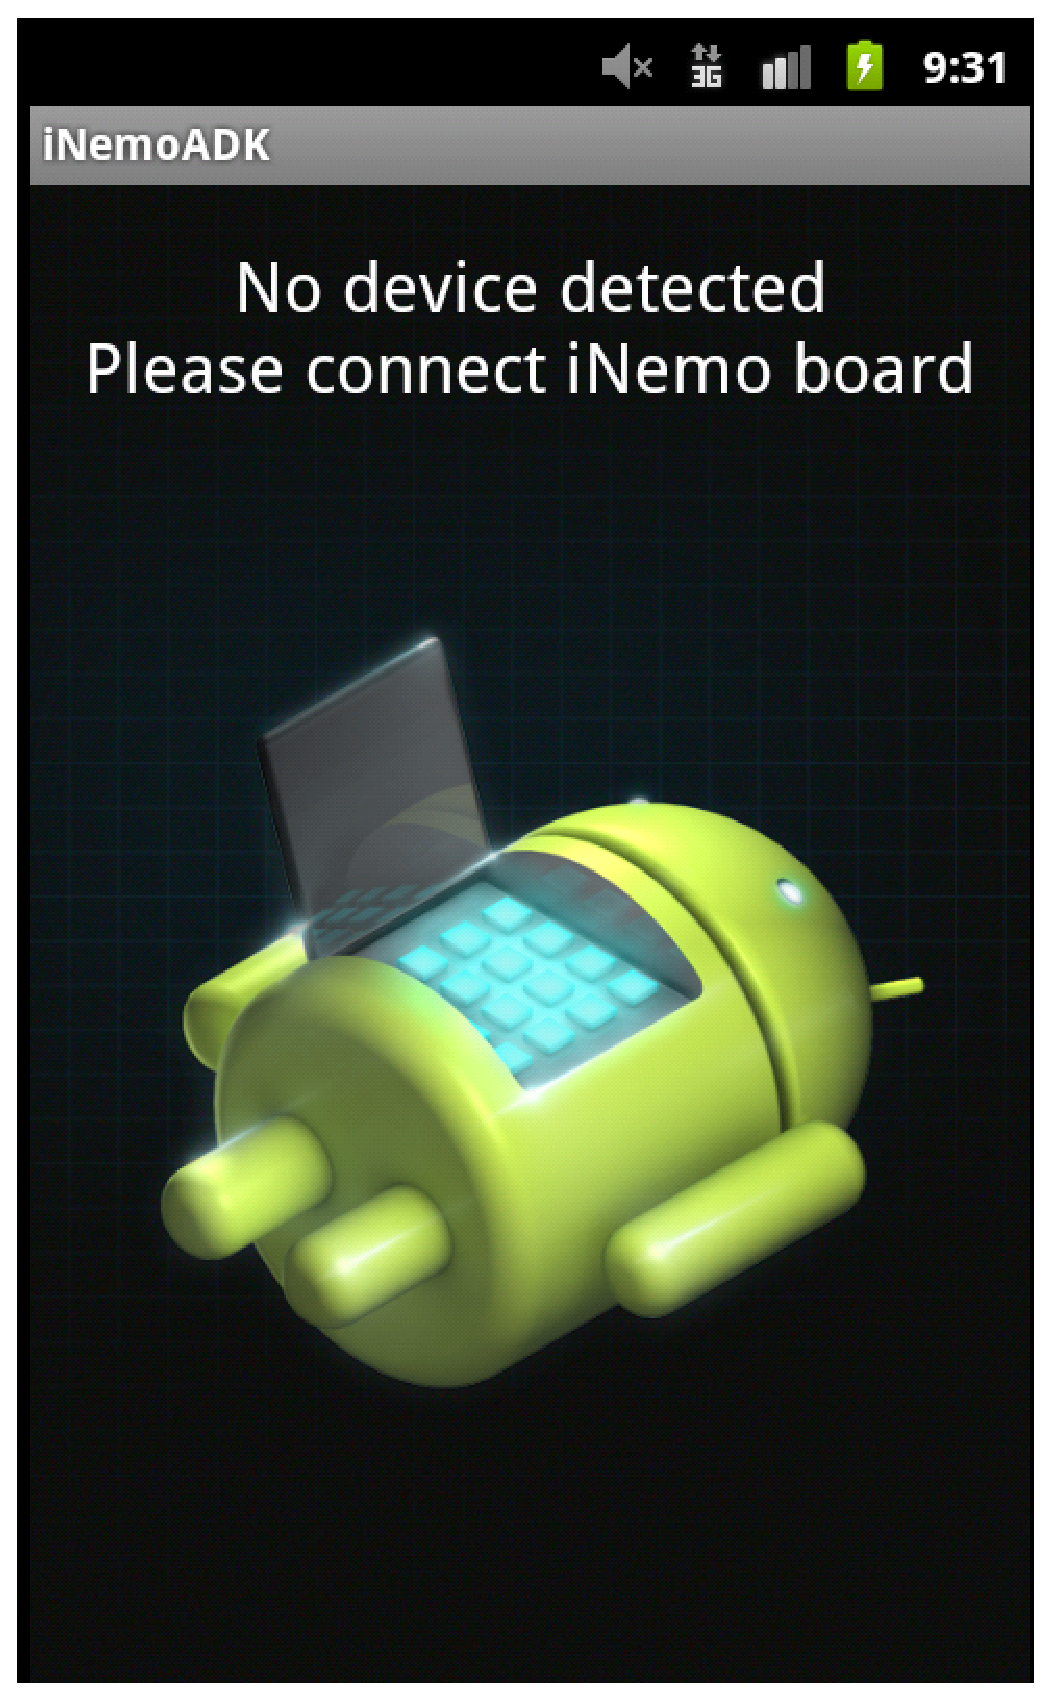
\includegraphics[width=0.6\linewidth]{pics/no_dev.eps}
	\captionof{figure}{Splash screen shown when the iNEMO board is detached.}
	\label{fig:no_dev}
\end{center}

When the board is attached, some introductive information on the board is shown and the user has the possibility to start the connection (see {\bf Figure \ref{fig:connect}}).

\begin{center}
	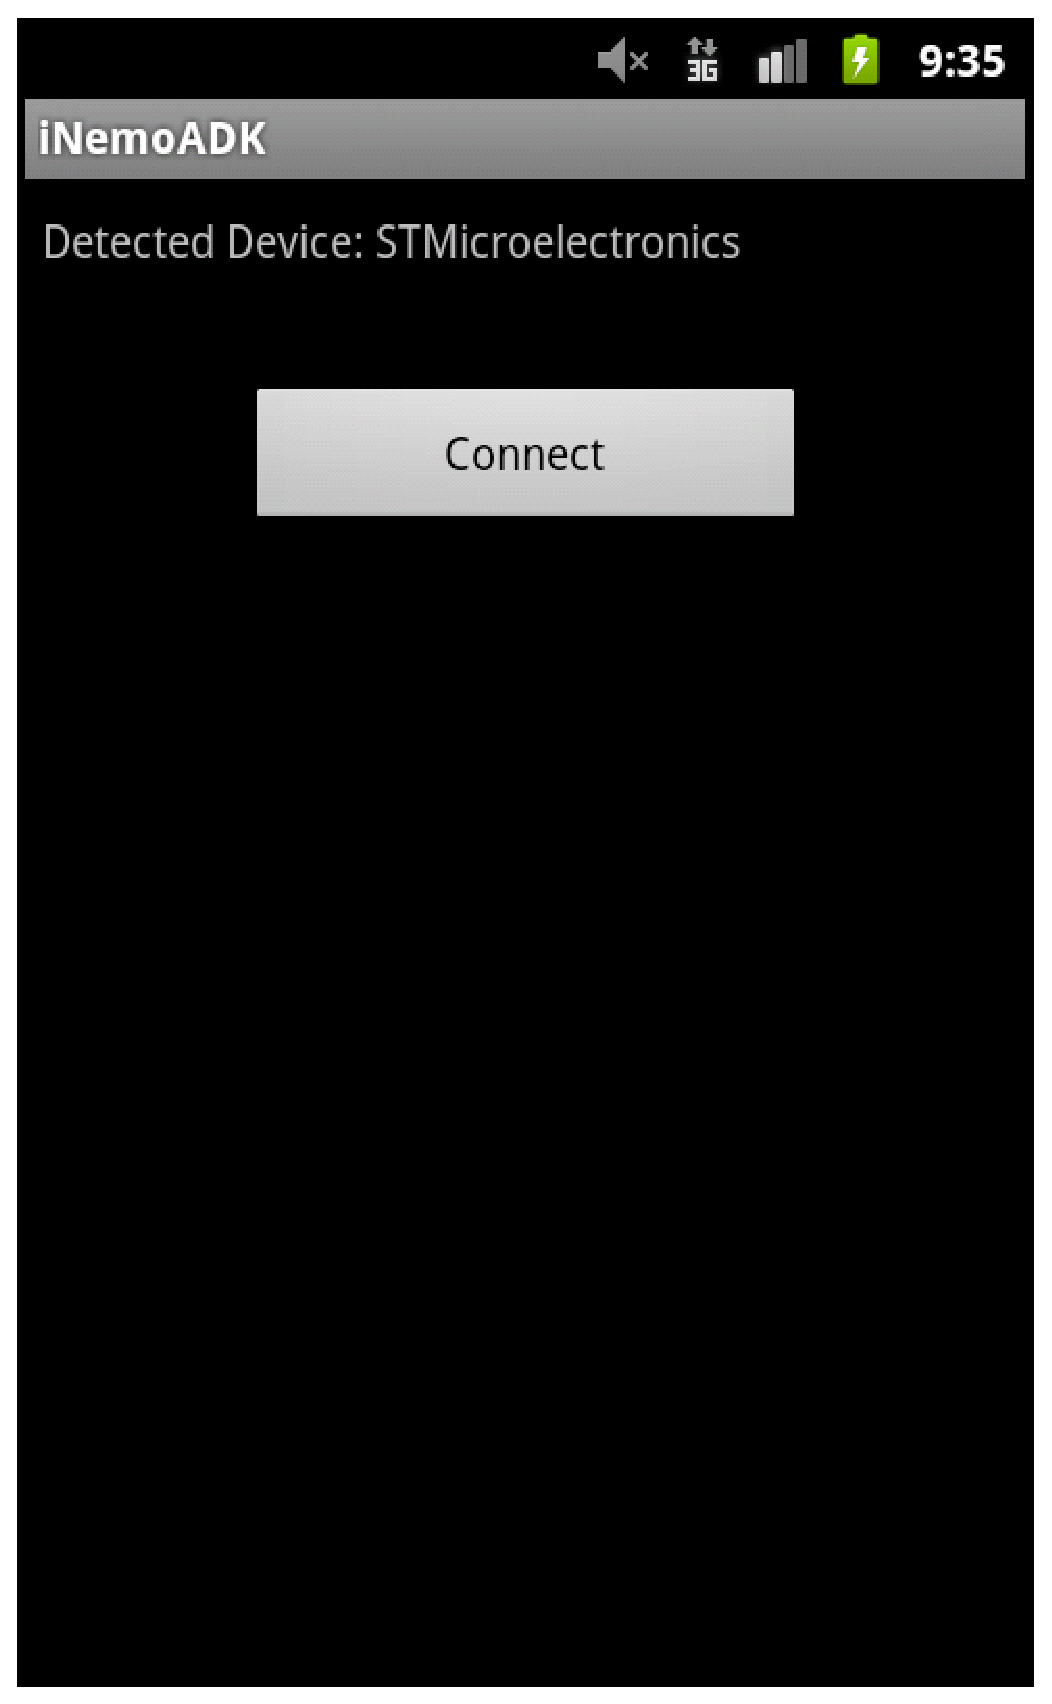
\includegraphics[width=0.6\linewidth]{pics/connect.eps}
	\captionof{figure}{Screen shown when the iNEMO board is attached.}
	\label{fig:connect}
\end{center}

When the connection is established, the application retrieves from the board information about the device identifier, the firmware and hardware version, the acquisition parameters and the sensors enabled. The user has the possibility to disconnect from the board, modify the acquisition parameters or start the acquisition (see {\bf Figure \ref{fig:connected}}).

\begin{center}
	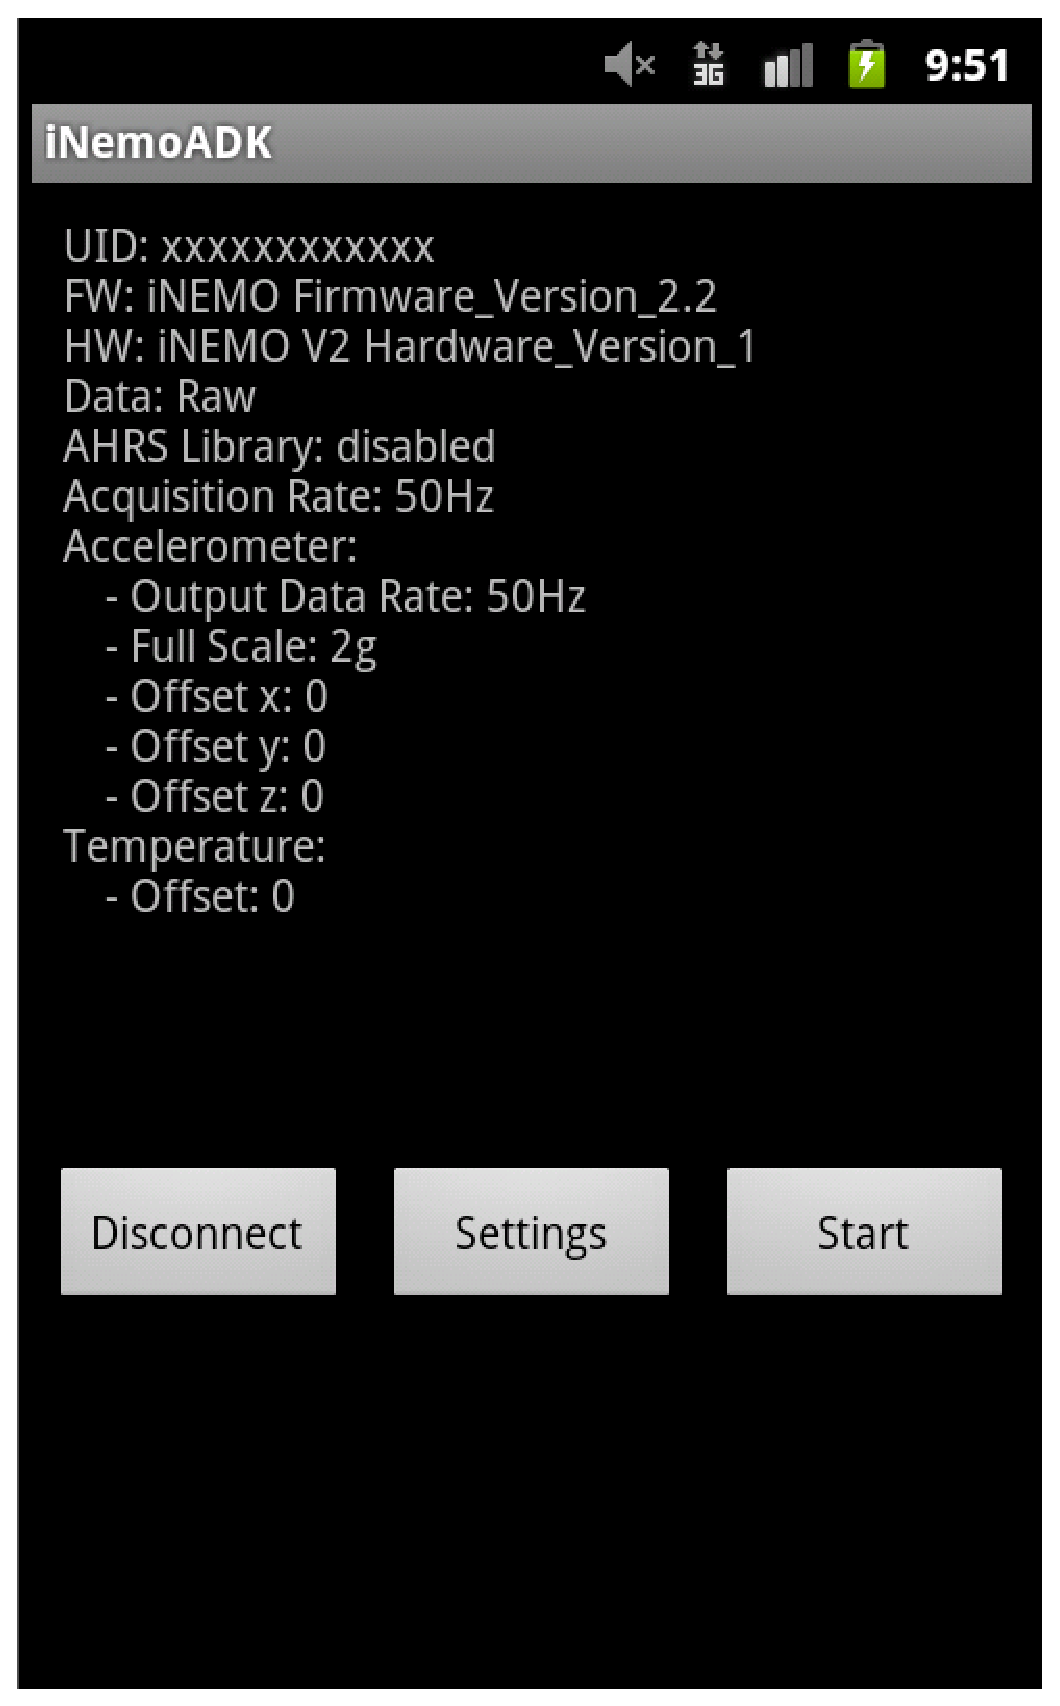
\includegraphics[width=0.6\linewidth]{pics/connected.eps}
	\captionof{figure}{Screen shown when the connection with the board is established.}
	\label{fig:connected}
\end{center}

The settings view ({\bf Figure \ref{fig:settings}}) allows the user to modify the acquisition parameters and to choose which sensors have to be enabled.

\begin{center}
	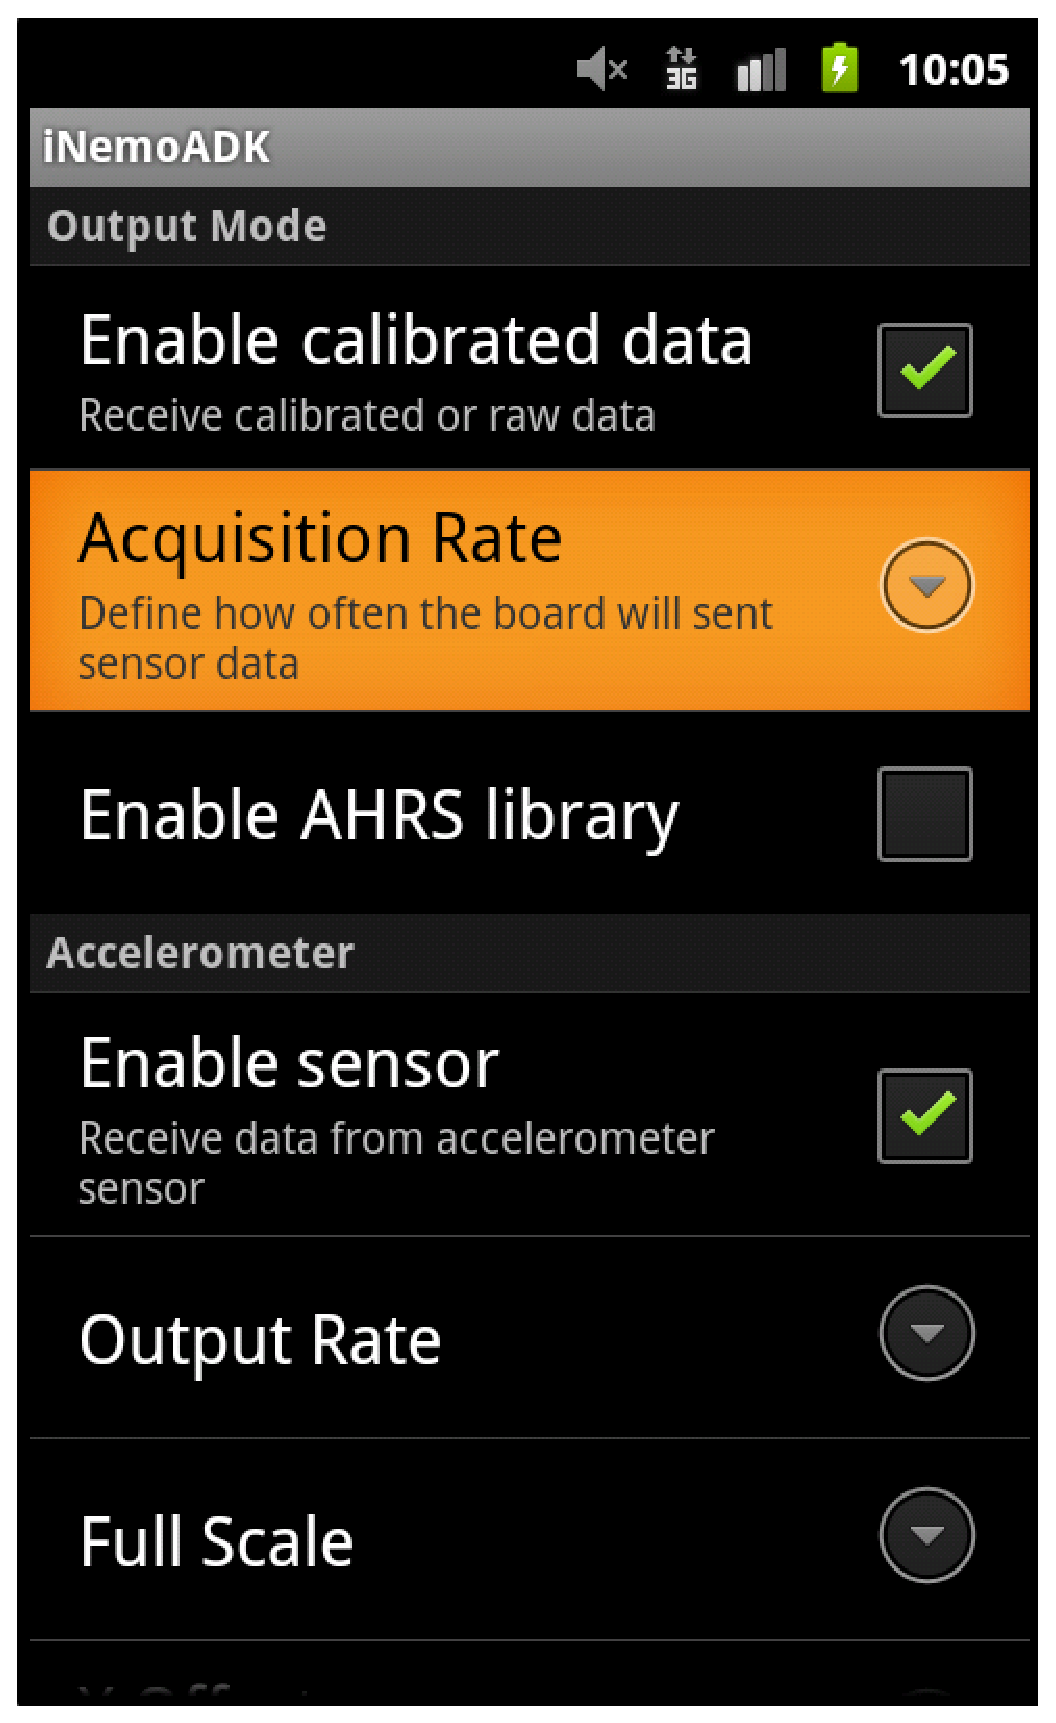
\includegraphics[width=0.6\linewidth]{pics/settings.eps}
	\captionof{figure}{Settings view.}
	\label{fig:settings}
\end{center}

Finally, during the acquisition phase, the application retrieves the data originated by the sensors of the board and shows them in a textual way (see {\bf Figure \ref{fig:acquisition}}). A future development is to shows sensor data in a graphical way (sliding graphs as in the Windows application iNEMO Suite).

\begin{center}
	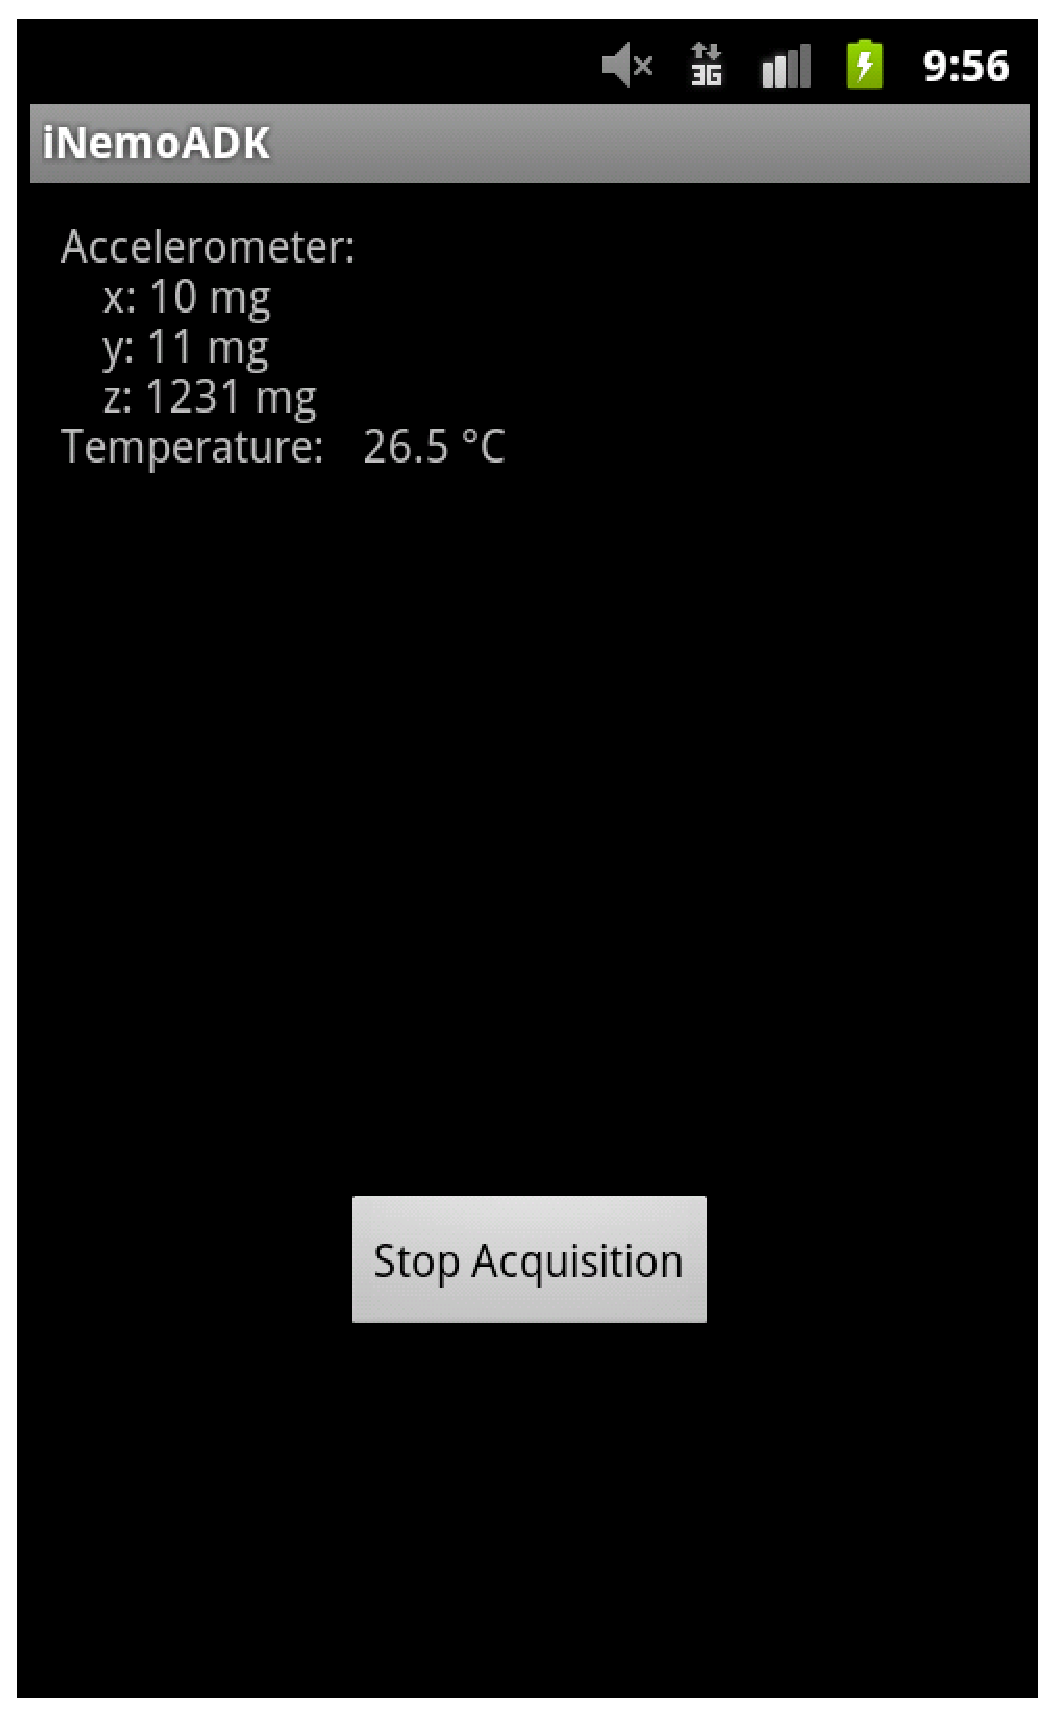
\includegraphics[width=0.6\linewidth]{pics/acquisition.eps}
	\captionof{figure}{Acquisition view.}
	\label{fig:acquisition}
\end{center}

As can be noticed, the layout is quite basic: another future development is to improve the graphic of the application.



\section{Conclusions}
\label{conclusions}

The results obtained with this work can be summarized as follows:

\begin{itemize}
	\item Added the support of Android Open ADK to STM32 microcontrollers' family.
	\item Defined a communication protocol for the exchange of messages between the iNEMO board and the Android device.
	\item Implemented the communication protocol both in the firmware and in the Android application.
	\item Implemented a set of task in the firmware that guarantees a correct communication with the Android device.
	\item Implemented a complete Android application that can establish a communication with the iNEMO board and show to the user the data originated from the sensors integrated on the board (for now in a textual way). The user can also change the acquisition parameters and choose which sensors have to be monitored.
\end{itemize}


Future developments for this work:

\begin{itemize}
	\item Show the data originated from the sensors in a graphical way (sliding graphs as in the Windows application iNEMO Suite).
	\item Implement a complete compilation chain based on gcc and Makefile, in order to get rid of the limitations imposed by Keil uVision IDE.
	\item Improve the graphic of the application.
\end{itemize}


%%%%%%%%%%%%%%%%%%%%%%%%%%%%%%%%%%%%%%%%%%%%%%%%%%%%%%%%%%%%%%%%%%%%%%%%%%%%%

% We suggest the use of JabRef for editing your bibliography file (Report.bib)
%\bibliographystyle{splncs}
\nocite{*}
\bibliographystyle{ieeetr}
\bibliography{Report}

\end{multicols}
\end{document}
